\begin{equation}
    - \Sigma^{\text{Hartree}}_{\vb*{k} \sigma \omega} = \begin{gathered}
        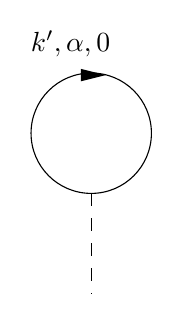
\begin{tikzpicture}[x=0.75pt,y=0.75pt,yscale=-1,xscale=1]
            %uncomment if require: \path (0,300); %set diagram left start at 0, and has height of 300
            
            %Straight Lines [id:da7796585827567135] 
            \draw  [dash pattern={on 4.5pt off 4.5pt}]  (247.35,162.98) -- (247.35,211) ;
            %Shape: Circle [id:dp5603225998122126] 
            \draw   (218.35,133.98) .. controls (218.35,117.96) and (231.34,104.98) .. (247.35,104.98) .. controls (263.37,104.98) and (276.35,117.96) .. (276.35,133.98) .. controls (276.35,150) and (263.37,162.98) .. (247.35,162.98) .. controls (231.34,162.98) and (218.35,150) .. (218.35,133.98) -- cycle ;
            %Straight Lines [id:da24340217870718206] 
            \draw    (254.35,105.98) ;
            \draw [shift={(254.35,105.98)}, rotate = 180] [fill={rgb, 255:red, 0; green, 0; blue, 0 }  ][line width=0.08]  [draw opacity=0] (12,-3) -- (0,0) -- (12,3) -- cycle    ;
            
            % Text Node
            \draw (217,83.4) node [anchor=north west][inner sep=0.75pt]    {$\boldsymbol{k} ',\alpha ,0$};
            \end{tikzpicture}      
   \end{gathered} = \frac{1}{V} \sum_{\vb*{k}', \alpha} (- V_0) n_{\vb*{k}' \alpha}^0,
   \label{eq:lowerest-self-energy-hartree-fermi-liquid}
\end{equation}